
%% 「。」を「.」にしたり、「、」を「,」にしたりするのは後で置換で一括でやります。

ドメイン適応は、大量のラベルデータの不足に対処するための新たな学習手法であり、転移学習の特殊なケースとして位置づけられる。
前節の定義に従うと、ドメイン適応は転移学習の中でも特に$D_S \neq D_T$であるものを指す。

本節では、Wanら\cite{wang2018deep}の論文による分類を元に、特に深層学習に注目して、ドメイン適応の定義と分類を示した後に、医療画像レジストレーションタスクがドメイン適応においてどのように分類されるのかを示す。

\subsection{ドメイン適応の分類}
    深層学習のような手法を用いない場合、ドメイン適応のアルゴリズムは2つに大別できる。
    1つ目は、ソースドメインでのラベルをターゲットドメインで利用するために、ソースドメインのデータ自体に重み付けをするような転移学習(Instance Transfer)である。
    2つ目は、ソースドメインおよびターゲットドメインの差や、モデル誤差を軽減する特徴量を見つけるような転移学習(Feature representation transfer)である。

    深層学習におけるドメイン適応を考慮する際に、このドメインの違いについての形態は、 それぞれのドメインが同質であるかどうかによってさらに2つに分類することが可能である。
    先述したように、ドメイン適応は転移学習の特殊なケースとして位置づけられ、$D_S \neq D_T$の場合を想定している。
    しかし、この定義ではこの差異がデータの分布によるものなのか、特徴空間の差異のことなのかは明確にされていない。
    そこで、、Wanら\cite{wang2018deep}はデータ分布のみが異なり、特徴空間は同一である場合をHomogeneous DA、特徴空間自体が異なる場合をHeterogeneous DAとして分類している。
    
    Heterogeneous DAは特徴空間自体が異なる場合であるが、取り扱うメディア自体が同じ場合と異なる場合でさらに2種類に分けることができる。
    取り扱うメディア自体が同じ(例:画像対画像)場合は、例えばデータ取得に利用したデバイスの差(可視光、近赤外、奥行き付映像など)や、画像スタイルの差異(絵と写真など)などのケースが考えられ、取り扱うメディア自体が異なる場合(例:画像対言語)には、メディアが同じ場合よりもドメインの差異が非常に大きくなる。

    深層学習モデルにおけるドメイン適応を考慮する際には、基本的にInstance Transferのような手法について議論されることは少ない。
    深層学習モデルをどのように設計すれば異なるドメインの表現を獲得することが可能かを議論することが大半であり、本論文ではこのような汎用的な特徴表現を学習することを前提としてドメイン適応を分類する。
    具体的には、データの種類によって学習の方法は「教師あり学習」「半教師あり学習」「教師なし学習」の3つに大別することができる。
    つまり、深層学習のOne-Stepドメイン適応は、ドメインの質に関して2通り、学習方法に関して3通りの分岐が存在し、合計で6つに分類することが可能であることが分かる(図\ref{category_of_DA})。
    
    \begin{figure}[ht]
      \centering
      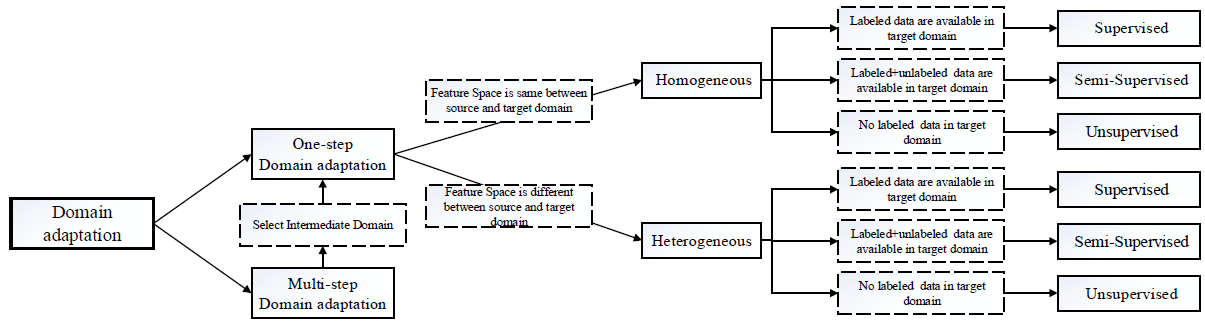
\includegraphics[width=\linewidth]{2_related_works/img/category_of_DA.png}
      \caption{An overview of different settings of domain adaptation\cite{wang2018deep}.}
      \label{category_of_DA}
    \end{figure}

    また、ドメインの特性が互いにあまりにも違う場合には、稀に中間のドメインを経由してドメイン適応を行う例(Multi-Step Domain Adaptation)も存在するが、本論文ではそのような例は扱わない。
    

\subsection{ドメイン適応のアプローチ}
    深層学習モデルをドメイン適応させるために、様々なアプローチが考案されている。
    これらのアプローチは大きく分けて3つに分類することができる\cite{csurka2017domain}。
    \subsubsection{Discrepancy base}
        discrepancyベースのアプローチは、教師データを用いて深層学習モデルを最適化する中でドメインシフトに対応する手法である。
        
        用いる損失関数や何を基準にするかによってさらに細分化されるが、多くが通常の深層学習モデルの訓練と同様に訓練が可能である。
        
        
        
        
    \subsubsection{Adversarial base}
        Adversarialベースのアプローチは、GANを用いてドメインの混合を促す手法である。
    \subsubsection{Reconstruction base}
        Reconstructionベースのアプローチは、補助的なタスクとして画像再構成を課すことにより、特徴量の普遍性を確保することを目指す手法である。
    
\subsection{医療画像におけるドメイン適応}
    医療画像におけるドメイン適応は、


\subsection{本論文におけるドメイン適応}
    本論文では、転移学習の中でも特にドメイン適応に焦点を当てる。
    すなわち、想定するのは$D_S \neq D_T$である状態であり、転移対象に関してはモデルのパラメータを想定する。
    %これはMR-CTなど、画像モダリティの違いを指す。
    基本的に後に述べる敵対的手法\cite{goodfellow2014generative}を用いてモデルを訓練することによりパラメータのドメイン適応を行い、2つのドメインに共通して利用できるモデルを作成することを目標とする。
    つまり、転移学習の枠組みにおいて、本研究はFeature-representation-transferを用いて伝達転移学習を行うことに焦点を当てている。
    しかし、ラベルの有無などの点で細かい定義から多少外れていることに注意されたい。
    次節ではドメイン適応について詳しく述べる。